\documentclass[twoside]{book}

% Packages required by doxygen
\usepackage{fixltx2e}
\usepackage{calc}
\usepackage{doxygen}
\usepackage[export]{adjustbox} % also loads graphicx
\usepackage{graphicx}
\usepackage[utf8]{inputenc}
\usepackage{makeidx}
\usepackage{multicol}
\usepackage{multirow}
\PassOptionsToPackage{warn}{textcomp}
\usepackage{textcomp}
\usepackage[nointegrals]{wasysym}
\usepackage[table]{xcolor}

% NLS support packages
\usepackage[french]{babel}

% Font selection
\usepackage[T1]{fontenc}
\usepackage[scaled=.90]{helvet}
\usepackage{courier}
\usepackage{amssymb}
\usepackage{sectsty}
\renewcommand{\familydefault}{\sfdefault}
\allsectionsfont{%
  \fontseries{bc}\selectfont%
  \color{darkgray}%
}
\renewcommand{\DoxyLabelFont}{%
  \fontseries{bc}\selectfont%
  \color{darkgray}%
}
\newcommand{\+}{\discretionary{\mbox{\scriptsize$\hookleftarrow$}}{}{}}

% Page & text layout
\usepackage{geometry}
\geometry{%
  a4paper,%
  top=2.5cm,%
  bottom=2.5cm,%
  left=2.5cm,%
  right=2.5cm%
}
\tolerance=750
\hfuzz=15pt
\hbadness=750
\setlength{\emergencystretch}{15pt}
\setlength{\parindent}{0cm}
\setlength{\parskip}{3ex plus 2ex minus 2ex}
\makeatletter
\renewcommand{\paragraph}{%
  \@startsection{paragraph}{4}{0ex}{-1.0ex}{1.0ex}{%
    \normalfont\normalsize\bfseries\SS@parafont%
  }%
}
\renewcommand{\subparagraph}{%
  \@startsection{subparagraph}{5}{0ex}{-1.0ex}{1.0ex}{%
    \normalfont\normalsize\bfseries\SS@subparafont%
  }%
}
\makeatother

% Headers & footers
\usepackage{fancyhdr}
\pagestyle{fancyplain}
\fancyhead[LE]{\fancyplain{}{\bfseries\thepage}}
\fancyhead[CE]{\fancyplain{}{}}
\fancyhead[RE]{\fancyplain{}{\bfseries\leftmark}}
\fancyhead[LO]{\fancyplain{}{\bfseries\rightmark}}
\fancyhead[CO]{\fancyplain{}{}}
\fancyhead[RO]{\fancyplain{}{\bfseries\thepage}}
\fancyfoot[LE]{\fancyplain{}{}}
\fancyfoot[CE]{\fancyplain{}{}}
\fancyfoot[RE]{\fancyplain{}{\bfseries\scriptsize Généré par Doxygen }}
\fancyfoot[LO]{\fancyplain{}{\bfseries\scriptsize Généré par Doxygen }}
\fancyfoot[CO]{\fancyplain{}{}}
\fancyfoot[RO]{\fancyplain{}{}}
\renewcommand{\footrulewidth}{0.4pt}
\renewcommand{\chaptermark}[1]{%
  \markboth{#1}{}%
}
\renewcommand{\sectionmark}[1]{%
  \markright{\thesection\ #1}%
}

% Indices & bibliography
\usepackage{natbib}
\usepackage[titles]{tocloft}
\setcounter{tocdepth}{3}
\setcounter{secnumdepth}{5}
\makeindex

% Hyperlinks (required, but should be loaded last)
\usepackage{ifpdf}
\ifpdf
  \usepackage[pdftex,pagebackref=true]{hyperref}
\else
  \usepackage[ps2pdf,pagebackref=true]{hyperref}
\fi
\hypersetup{%
  colorlinks=true,%
  linkcolor=blue,%
  citecolor=blue,%
  unicode%
}

% Custom commands
\newcommand{\clearemptydoublepage}{%
  \newpage{\pagestyle{empty}\cleardoublepage}%
}

\usepackage{caption}
\captionsetup{labelsep=space,justification=centering,font={bf},singlelinecheck=off,skip=4pt,position=top}

%===== C O N T E N T S =====

\begin{document}

% Titlepage & ToC
\hypersetup{pageanchor=false,
             bookmarksnumbered=true,
             pdfencoding=unicode
            }
\pagenumbering{alph}
\begin{titlepage}
\vspace*{7cm}
\begin{center}%
{\Large Application\+\_\+\+Swipe \\[1ex]\large 1.\+1.\+1 }\\
\vspace*{1cm}
{\large Généré par Doxygen 1.8.13}\\
\end{center}
\end{titlepage}
\clearemptydoublepage
\pagenumbering{roman}
\tableofcontents
\clearemptydoublepage
\pagenumbering{arabic}
\hypersetup{pageanchor=true}

%--- Begin generated contents ---
\chapter{Index hiérarchique}
\section{Hiérarchie des classes}
Cette liste d\textquotesingle{}héritage est classée approximativement par ordre alphabétique \+:\begin{DoxyCompactList}
\item Q\+Object\begin{DoxyCompactList}
\item \contentsline{section}{Base\+B\+DD}{\pageref{class_base_b_d_d}}{}
\end{DoxyCompactList}
\end{DoxyCompactList}

\chapter{Index des classes}
\section{Liste des classes}
Liste des classes, structures, unions et interfaces avec une brève description \+:\begin{DoxyCompactList}
\item\contentsline{section}{\hyperlink{class_base_b_d_d}{Base\+B\+DD} }{\pageref{class_base_b_d_d}}{}
\end{DoxyCompactList}

\chapter{Index des fichiers}
\section{Liste des fichiers}
Liste de tous les fichiers avec une brève description \+:\begin{DoxyCompactList}
\item\contentsline{section}{/home/bmezerette/\+Documents/\+Github/\+Application\+\_\+\+Smartphone/\+Application\+\_\+\+Swipe\+\_\+\+Test\+\_\+\+Preliminaire/\hyperlink{basebdd_8cpp}{basebdd.\+cpp} }{\pageref{basebdd_8cpp}}{}
\item\contentsline{section}{/home/bmezerette/\+Documents/\+Github/\+Application\+\_\+\+Smartphone/\+Application\+\_\+\+Swipe\+\_\+\+Test\+\_\+\+Preliminaire/\hyperlink{basebdd_8h}{basebdd.\+h} }{\pageref{basebdd_8h}}{}
\item\contentsline{section}{/home/bmezerette/\+Documents/\+Github/\+Application\+\_\+\+Smartphone/\+Application\+\_\+\+Swipe\+\_\+\+Test\+\_\+\+Preliminaire/\hyperlink{main_8cpp}{main.\+cpp} }{\pageref{main_8cpp}}{}
\end{DoxyCompactList}

\chapter{Documentation des classes}
\hypertarget{class_base_b_d_d}{}\section{Référence de la classe Base\+B\+DD}
\label{class_base_b_d_d}\index{Base\+B\+DD@{Base\+B\+DD}}


{\ttfamily \#include $<$basebdd.\+h$>$}



Graphe d\textquotesingle{}héritage de Base\+B\+DD\+:
\nopagebreak
\begin{figure}[H]
\begin{center}
\leavevmode
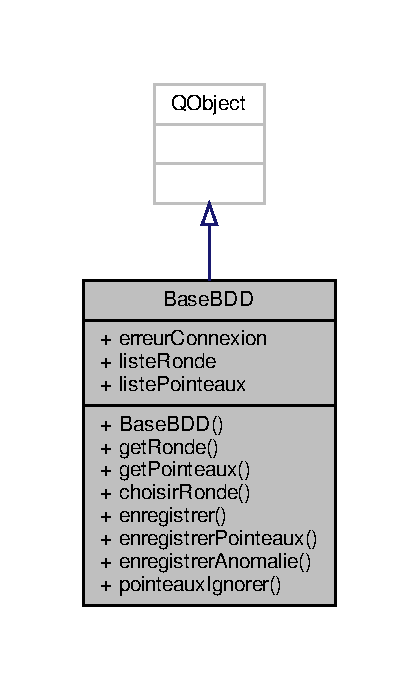
\includegraphics[width=201pt]{class_base_b_d_d__inherit__graph}
\end{center}
\end{figure}


Graphe de collaboration de Base\+B\+DD\+:
\nopagebreak
\begin{figure}[H]
\begin{center}
\leavevmode
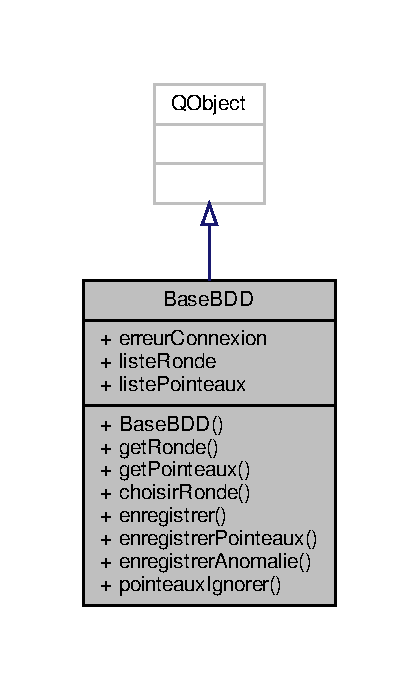
\includegraphics[width=201pt]{class_base_b_d_d__coll__graph}
\end{center}
\end{figure}
\subsection*{Signaux}
\begin{DoxyCompactItemize}
\item 
void \hyperlink{class_base_b_d_d_af25fa79519e164584eea311acafd51e7}{erreur\+Changed} ()
\begin{DoxyCompactList}\small\item\em Permet de recuperer id\+Ronde de la ronde choisie. \end{DoxyCompactList}\item 
void \hyperlink{class_base_b_d_d_a0e86919a03af0f469f351ea215f76340}{liste\+Ronde\+Changed} ()
\item 
void \hyperlink{class_base_b_d_d_aef78a59308e7f9ee23dfb62e7664d57a}{liste\+Pointeaux\+Changed} ()
\end{DoxyCompactItemize}
\subsection*{Fonctions membres publiques}
\begin{DoxyCompactItemize}
\item 
\hyperlink{class_base_b_d_d_ae9e4c871c20e159acbd08a97a7a6aa45}{Base\+B\+DD} (Q\+Object $\ast$parent=nullptr)
\begin{DoxyCompactList}\small\item\em Affiche la liste des pointeaux dans le combobox. \end{DoxyCompactList}\item 
Q\+String\+List \hyperlink{class_base_b_d_d_ad72a05677ec0613187ede9eb08f921b9}{get\+Ronde} ()
\begin{DoxyCompactList}\small\item\em \hyperlink{class_base_b_d_d_ad72a05677ec0613187ede9eb08f921b9}{Base\+B\+D\+D\+::get\+Ronde} Cette fonction permet de recuperer le nom des rondes. \end{DoxyCompactList}\item 
Q\+String\+List \hyperlink{class_base_b_d_d_ab5db945df6714aca26fe5b0eaa629c66}{get\+Pointeaux} ()
\begin{DoxyCompactList}\small\item\em \hyperlink{class_base_b_d_d_ab5db945df6714aca26fe5b0eaa629c66}{Base\+B\+D\+D\+::get\+Pointeaux} Cette fonction permet de recuperer tous d\textquotesingle{}abord l\textquotesingle{}id de la ronde. et ensuite grâce à l\textquotesingle{}id de la ronde ensuite recuperer les pointeaux de la ronde. \end{DoxyCompactList}\item 
Q\+\_\+\+I\+N\+V\+O\+K\+A\+B\+LE bool \hyperlink{class_base_b_d_d_aaf97d5447c9e64403c95458630434b7a}{choisir\+Ronde} (Q\+String \+\_\+nom\+Ronde)
\begin{DoxyCompactList}\small\item\em \hyperlink{class_base_b_d_d_aaf97d5447c9e64403c95458630434b7a}{Base\+B\+D\+D\+::choisir\+Ronde}. \end{DoxyCompactList}\item 
Q\+\_\+\+I\+N\+V\+O\+K\+A\+B\+LE void \hyperlink{class_base_b_d_d_a90699f331825ff764a578233a45a2d17}{enregistrer} (const Q\+String \+\_\+donnee\+B\+DD)
\begin{DoxyCompactList}\small\item\em Permet de recuperer le nom de la ronde choisie. \end{DoxyCompactList}\item 
Q\+\_\+\+I\+N\+V\+O\+K\+A\+B\+LE void \hyperlink{class_base_b_d_d_a52ff865a9fc36b11a9c2cbdb8cd9daa1}{enregistrer\+Pointeaux} (const Q\+String \+\_\+donnee\+B\+DD)
\begin{DoxyCompactList}\small\item\em Permet d\textquotesingle{}enregistrer dans la table Historique\+Pointeaux id\+Agent,nom\+Pointeau,date,anomalie. \end{DoxyCompactList}\item 
Q\+\_\+\+I\+N\+V\+O\+K\+A\+B\+LE void \hyperlink{class_base_b_d_d_a9c5f51c11f49e494e608a9dafb635629}{enregistrer\+Anomalie} (const Q\+String \+\_\+donnee\+Anomalie)
\begin{DoxyCompactList}\small\item\em Permet de récuperer le nom du pointeau actuel. \end{DoxyCompactList}\item 
Q\+\_\+\+I\+N\+V\+O\+K\+A\+B\+LE void \hyperlink{class_base_b_d_d_acbdf1ddaaaff9fa469ecef3a14ef1081}{pointeaux\+Ignorer} ()
\begin{DoxyCompactList}\small\item\em Permet d\textquotesingle{}enregistrer l\textquotesingle{}anomalie dans la B\+DD. \end{DoxyCompactList}\end{DoxyCompactItemize}
\subsection*{Propriétés}
\begin{DoxyCompactItemize}
\item 
bool \hyperlink{class_base_b_d_d_a11fdd43781eea1fe6f9b9b91d83a4a64}{erreur\+Connexion}
\item 
Q\+String\+List \hyperlink{class_base_b_d_d_abb6ff92708dd4be7304be2b3e74930c4}{liste\+Ronde}
\begin{DoxyCompactList}\small\item\em Si il y a une erreur D\textquotesingle{}ouverture de la B\+DD. \end{DoxyCompactList}\item 
Q\+String\+List \hyperlink{class_base_b_d_d_a706e89c393728daa3478dfe83208489c}{liste\+Pointeaux}
\begin{DoxyCompactList}\small\item\em Affiche la liste des rondes dans le combobox. \end{DoxyCompactList}\end{DoxyCompactItemize}


\subsection{Documentation des constructeurs et destructeur}
\mbox{\Hypertarget{class_base_b_d_d_ae9e4c871c20e159acbd08a97a7a6aa45}\label{class_base_b_d_d_ae9e4c871c20e159acbd08a97a7a6aa45}} 
\index{Base\+B\+DD@{Base\+B\+DD}!Base\+B\+DD@{Base\+B\+DD}}
\index{Base\+B\+DD@{Base\+B\+DD}!Base\+B\+DD@{Base\+B\+DD}}
\subsubsection{\texorpdfstring{Base\+B\+D\+D()}{BaseBDD()}}
{\footnotesize\ttfamily Base\+B\+D\+D\+::\+Base\+B\+DD (\begin{DoxyParamCaption}\item[{Q\+Object $\ast$}]{parent = {\ttfamily nullptr} }\end{DoxyParamCaption})\hspace{0.3cm}{\ttfamily [explicit]}}



Affiche la liste des pointeaux dans le combobox. 

\hyperlink{class_base_b_d_d_ae9e4c871c20e159acbd08a97a7a6aa45}{Base\+B\+D\+D\+::\+Base\+B\+DD}.


\begin{DoxyParams}{Paramètres}
{\em parent} & Le constructeur permet d\textquotesingle{}ouvrir la B\+DD et si elle ne s\textquotesingle{}ouvre pas elle emet un signal qui appelleras la fonction erreur\+Connexion. \\
\hline
\end{DoxyParams}


\subsection{Documentation des fonctions membres}
\mbox{\Hypertarget{class_base_b_d_d_aaf97d5447c9e64403c95458630434b7a}\label{class_base_b_d_d_aaf97d5447c9e64403c95458630434b7a}} 
\index{Base\+B\+DD@{Base\+B\+DD}!choisir\+Ronde@{choisir\+Ronde}}
\index{choisir\+Ronde@{choisir\+Ronde}!Base\+B\+DD@{Base\+B\+DD}}
\subsubsection{\texorpdfstring{choisir\+Ronde()}{choisirRonde()}}
{\footnotesize\ttfamily bool Base\+B\+D\+D\+::choisir\+Ronde (\begin{DoxyParamCaption}\item[{Q\+String}]{\+\_\+nom\+Ronde }\end{DoxyParamCaption})}



\hyperlink{class_base_b_d_d_aaf97d5447c9e64403c95458630434b7a}{Base\+B\+D\+D\+::choisir\+Ronde}. 


\begin{DoxyParams}{Paramètres}
{\em \+\_\+nom\+Ronde} & sert a récuperer le nom de la ronde actuelle Choisir\+Ronde permet de recuperer le Ronde choisie. \\
\hline
\end{DoxyParams}
\begin{DoxyReturn}{Renvoie}

\end{DoxyReturn}
\mbox{\Hypertarget{class_base_b_d_d_a90699f331825ff764a578233a45a2d17}\label{class_base_b_d_d_a90699f331825ff764a578233a45a2d17}} 
\index{Base\+B\+DD@{Base\+B\+DD}!enregistrer@{enregistrer}}
\index{enregistrer@{enregistrer}!Base\+B\+DD@{Base\+B\+DD}}
\subsubsection{\texorpdfstring{enregistrer()}{enregistrer()}}
{\footnotesize\ttfamily void Base\+B\+D\+D\+::enregistrer (\begin{DoxyParamCaption}\item[{const Q\+String}]{\+\_\+donnee\+B\+DD }\end{DoxyParamCaption})}



Permet de recuperer le nom de la ronde choisie. 

\hyperlink{class_base_b_d_d_a90699f331825ff764a578233a45a2d17}{Base\+B\+D\+D\+::enregistrer}.


\begin{DoxyParams}{Paramètres}
{\em \+\_\+donnee\+B\+DD} & contient le nom\+Pointeaux de notre combobox La fonction enregistrer permet enregistrer les scannes de nos pointeaux tous au long de notre ronde. \\
\hline
\end{DoxyParams}
\mbox{\Hypertarget{class_base_b_d_d_a9c5f51c11f49e494e608a9dafb635629}\label{class_base_b_d_d_a9c5f51c11f49e494e608a9dafb635629}} 
\index{Base\+B\+DD@{Base\+B\+DD}!enregistrer\+Anomalie@{enregistrer\+Anomalie}}
\index{enregistrer\+Anomalie@{enregistrer\+Anomalie}!Base\+B\+DD@{Base\+B\+DD}}
\subsubsection{\texorpdfstring{enregistrer\+Anomalie()}{enregistrerAnomalie()}}
{\footnotesize\ttfamily void Base\+B\+D\+D\+::enregistrer\+Anomalie (\begin{DoxyParamCaption}\item[{const Q\+String}]{\+\_\+donnee\+Anomalie }\end{DoxyParamCaption})}



Permet de récuperer le nom du pointeau actuel. 

\hyperlink{class_base_b_d_d_a9c5f51c11f49e494e608a9dafb635629}{Base\+B\+D\+D\+::enregistrer\+Anomalie}.


\begin{DoxyParams}{Paramètres}
{\em \+\_\+donnee\+Anomalie} & permet de recuperer la description de l\textquotesingle{}anomalie qui se trouve dans le textfield de notre application. Qui nous serviras ensuite pour enregistrer l\textquotesingle{}anomalie dans la base de données tous en enregistrant le pointeaux actuelle avec l\textquotesingle{}heure aussi. \\
\hline
\end{DoxyParams}
\mbox{\Hypertarget{class_base_b_d_d_a52ff865a9fc36b11a9c2cbdb8cd9daa1}\label{class_base_b_d_d_a52ff865a9fc36b11a9c2cbdb8cd9daa1}} 
\index{Base\+B\+DD@{Base\+B\+DD}!enregistrer\+Pointeaux@{enregistrer\+Pointeaux}}
\index{enregistrer\+Pointeaux@{enregistrer\+Pointeaux}!Base\+B\+DD@{Base\+B\+DD}}
\subsubsection{\texorpdfstring{enregistrer\+Pointeaux()}{enregistrerPointeaux()}}
{\footnotesize\ttfamily void Base\+B\+D\+D\+::enregistrer\+Pointeaux (\begin{DoxyParamCaption}\item[{const Q\+String}]{\+\_\+donnee\+B\+DD }\end{DoxyParamCaption})}



Permet d\textquotesingle{}enregistrer dans la table Historique\+Pointeaux id\+Agent,nom\+Pointeau,date,anomalie. 

\hyperlink{class_base_b_d_d_a52ff865a9fc36b11a9c2cbdb8cd9daa1}{Base\+B\+D\+D\+::enregistrer\+Pointeaux}.


\begin{DoxyParams}{Paramètres}
{\em \+\_\+donnee\+B\+DD} & recupère donc le nom du pointeaux actuelle pour que nom\+Pointeaux un attribut que n\textquotesingle{}importe qu\textquotesingle{}elle fonction peut avoir accès prenne cette valeur pour pouvoir ensuite le scanner, ce parametre seras utiliser dans la fonction \hyperlink{class_base_b_d_d_acbdf1ddaaaff9fa469ecef3a14ef1081}{pointeaux\+Ignorer()} et \hyperlink{class_base_b_d_d_a9c5f51c11f49e494e608a9dafb635629}{enregistrer\+Anomalie()}. \\
\hline
\end{DoxyParams}
\mbox{\Hypertarget{class_base_b_d_d_af25fa79519e164584eea311acafd51e7}\label{class_base_b_d_d_af25fa79519e164584eea311acafd51e7}} 
\index{Base\+B\+DD@{Base\+B\+DD}!erreur\+Changed@{erreur\+Changed}}
\index{erreur\+Changed@{erreur\+Changed}!Base\+B\+DD@{Base\+B\+DD}}
\subsubsection{\texorpdfstring{erreur\+Changed}{erreurChanged}}
{\footnotesize\ttfamily void Base\+B\+D\+D\+::erreur\+Changed (\begin{DoxyParamCaption}{ }\end{DoxyParamCaption})\hspace{0.3cm}{\ttfamily [signal]}}



Permet de recuperer id\+Ronde de la ronde choisie. 

\mbox{\Hypertarget{class_base_b_d_d_ab5db945df6714aca26fe5b0eaa629c66}\label{class_base_b_d_d_ab5db945df6714aca26fe5b0eaa629c66}} 
\index{Base\+B\+DD@{Base\+B\+DD}!get\+Pointeaux@{get\+Pointeaux}}
\index{get\+Pointeaux@{get\+Pointeaux}!Base\+B\+DD@{Base\+B\+DD}}
\subsubsection{\texorpdfstring{get\+Pointeaux()}{getPointeaux()}}
{\footnotesize\ttfamily Q\+String\+List Base\+B\+D\+D\+::get\+Pointeaux (\begin{DoxyParamCaption}{ }\end{DoxyParamCaption})}



\hyperlink{class_base_b_d_d_ab5db945df6714aca26fe5b0eaa629c66}{Base\+B\+D\+D\+::get\+Pointeaux} Cette fonction permet de recuperer tous d\textquotesingle{}abord l\textquotesingle{}id de la ronde. et ensuite grâce à l\textquotesingle{}id de la ronde ensuite recuperer les pointeaux de la ronde. 

\begin{DoxyReturn}{Renvoie}

\end{DoxyReturn}
\mbox{\Hypertarget{class_base_b_d_d_ad72a05677ec0613187ede9eb08f921b9}\label{class_base_b_d_d_ad72a05677ec0613187ede9eb08f921b9}} 
\index{Base\+B\+DD@{Base\+B\+DD}!get\+Ronde@{get\+Ronde}}
\index{get\+Ronde@{get\+Ronde}!Base\+B\+DD@{Base\+B\+DD}}
\subsubsection{\texorpdfstring{get\+Ronde()}{getRonde()}}
{\footnotesize\ttfamily Q\+String\+List Base\+B\+D\+D\+::get\+Ronde (\begin{DoxyParamCaption}{ }\end{DoxyParamCaption})}



\hyperlink{class_base_b_d_d_ad72a05677ec0613187ede9eb08f921b9}{Base\+B\+D\+D\+::get\+Ronde} Cette fonction permet de recuperer le nom des rondes. 

\mbox{\Hypertarget{class_base_b_d_d_aef78a59308e7f9ee23dfb62e7664d57a}\label{class_base_b_d_d_aef78a59308e7f9ee23dfb62e7664d57a}} 
\index{Base\+B\+DD@{Base\+B\+DD}!liste\+Pointeaux\+Changed@{liste\+Pointeaux\+Changed}}
\index{liste\+Pointeaux\+Changed@{liste\+Pointeaux\+Changed}!Base\+B\+DD@{Base\+B\+DD}}
\subsubsection{\texorpdfstring{liste\+Pointeaux\+Changed}{listePointeauxChanged}}
{\footnotesize\ttfamily void Base\+B\+D\+D\+::liste\+Pointeaux\+Changed (\begin{DoxyParamCaption}{ }\end{DoxyParamCaption})\hspace{0.3cm}{\ttfamily [signal]}}

\mbox{\Hypertarget{class_base_b_d_d_a0e86919a03af0f469f351ea215f76340}\label{class_base_b_d_d_a0e86919a03af0f469f351ea215f76340}} 
\index{Base\+B\+DD@{Base\+B\+DD}!liste\+Ronde\+Changed@{liste\+Ronde\+Changed}}
\index{liste\+Ronde\+Changed@{liste\+Ronde\+Changed}!Base\+B\+DD@{Base\+B\+DD}}
\subsubsection{\texorpdfstring{liste\+Ronde\+Changed}{listeRondeChanged}}
{\footnotesize\ttfamily void Base\+B\+D\+D\+::liste\+Ronde\+Changed (\begin{DoxyParamCaption}{ }\end{DoxyParamCaption})\hspace{0.3cm}{\ttfamily [signal]}}

\mbox{\Hypertarget{class_base_b_d_d_acbdf1ddaaaff9fa469ecef3a14ef1081}\label{class_base_b_d_d_acbdf1ddaaaff9fa469ecef3a14ef1081}} 
\index{Base\+B\+DD@{Base\+B\+DD}!pointeaux\+Ignorer@{pointeaux\+Ignorer}}
\index{pointeaux\+Ignorer@{pointeaux\+Ignorer}!Base\+B\+DD@{Base\+B\+DD}}
\subsubsection{\texorpdfstring{pointeaux\+Ignorer()}{pointeauxIgnorer()}}
{\footnotesize\ttfamily void Base\+B\+D\+D\+::pointeaux\+Ignorer (\begin{DoxyParamCaption}{ }\end{DoxyParamCaption})}



Permet d\textquotesingle{}enregistrer l\textquotesingle{}anomalie dans la B\+DD. 

\hyperlink{class_base_b_d_d_acbdf1ddaaaff9fa469ecef3a14ef1081}{Base\+B\+D\+D\+::pointeaux\+Ignorer} pointeaux\+Ignoré permet de ignoré le pointeaux actuelle si il ne fonctionne pas, donc dans la B\+DD dans le champ anomalie il seras écrit Pointeaux ignoré mais aussi sa va enregistré aussi id\+Agent, nom\+Pointeaux, date. 

\subsection{Documentation des propriétés}
\mbox{\Hypertarget{class_base_b_d_d_a11fdd43781eea1fe6f9b9b91d83a4a64}\label{class_base_b_d_d_a11fdd43781eea1fe6f9b9b91d83a4a64}} 
\index{Base\+B\+DD@{Base\+B\+DD}!erreur\+Connexion@{erreur\+Connexion}}
\index{erreur\+Connexion@{erreur\+Connexion}!Base\+B\+DD@{Base\+B\+DD}}
\subsubsection{\texorpdfstring{erreur\+Connexion}{erreurConnexion}}
{\footnotesize\ttfamily bool Base\+B\+D\+D\+::erreur\+Connexion}

\mbox{\Hypertarget{class_base_b_d_d_a706e89c393728daa3478dfe83208489c}\label{class_base_b_d_d_a706e89c393728daa3478dfe83208489c}} 
\index{Base\+B\+DD@{Base\+B\+DD}!liste\+Pointeaux@{liste\+Pointeaux}}
\index{liste\+Pointeaux@{liste\+Pointeaux}!Base\+B\+DD@{Base\+B\+DD}}
\subsubsection{\texorpdfstring{liste\+Pointeaux}{listePointeaux}}
{\footnotesize\ttfamily Q\+String\+List Base\+B\+D\+D\+::liste\+Pointeaux\hspace{0.3cm}{\ttfamily [read]}}



Affiche la liste des rondes dans le combobox. 

\mbox{\Hypertarget{class_base_b_d_d_abb6ff92708dd4be7304be2b3e74930c4}\label{class_base_b_d_d_abb6ff92708dd4be7304be2b3e74930c4}} 
\index{Base\+B\+DD@{Base\+B\+DD}!liste\+Ronde@{liste\+Ronde}}
\index{liste\+Ronde@{liste\+Ronde}!Base\+B\+DD@{Base\+B\+DD}}
\subsubsection{\texorpdfstring{liste\+Ronde}{listeRonde}}
{\footnotesize\ttfamily Q\+String\+List Base\+B\+D\+D\+::liste\+Ronde\hspace{0.3cm}{\ttfamily [read]}}



Si il y a une erreur D\textquotesingle{}ouverture de la B\+DD. 



La documentation de cette classe a été générée à partir des fichiers suivants \+:\begin{DoxyCompactItemize}
\item 
/home/bmezerette/\+Documents/\+Github/\+Application\+\_\+\+Smartphone/\+Application\+\_\+\+Swipe\+\_\+\+Test\+\_\+\+Preliminaire/\hyperlink{basebdd_8h}{basebdd.\+h}\item 
/home/bmezerette/\+Documents/\+Github/\+Application\+\_\+\+Smartphone/\+Application\+\_\+\+Swipe\+\_\+\+Test\+\_\+\+Preliminaire/\hyperlink{basebdd_8cpp}{basebdd.\+cpp}\end{DoxyCompactItemize}

\chapter{Documentation des fichiers}
\hypertarget{basebdd_8cpp}{}\section{Référence du fichier /home/bmezerette/\+Documents/\+Github/\+Application\+\_\+\+Smartphone/\+Application\+\_\+\+Swipe\+\_\+\+Test\+\_\+\+Preliminaire/basebdd.cpp}
\label{basebdd_8cpp}\index{/home/bmezerette/\+Documents/\+Github/\+Application\+\_\+\+Smartphone/\+Application\+\_\+\+Swipe\+\_\+\+Test\+\_\+\+Preliminaire/basebdd.\+cpp@{/home/bmezerette/\+Documents/\+Github/\+Application\+\_\+\+Smartphone/\+Application\+\_\+\+Swipe\+\_\+\+Test\+\_\+\+Preliminaire/basebdd.\+cpp}}
{\ttfamily \#include \char`\"{}basebdd.\+h\char`\"{}}\newline
{\ttfamily \#include \char`\"{}Q\+Debug\char`\"{}}\newline
{\ttfamily \#include $<$Qt\+Sql/\+Q\+Sql\+Error$>$}\newline
{\ttfamily \#include $<$Qt\+Sql/\+Q\+Sql\+Query$>$}\newline
{\ttfamily \#include $<$Q\+Message\+Box$>$}\newline
Graphe des dépendances par inclusion de basebdd.\+cpp\+:
\nopagebreak
\begin{figure}[H]
\begin{center}
\leavevmode
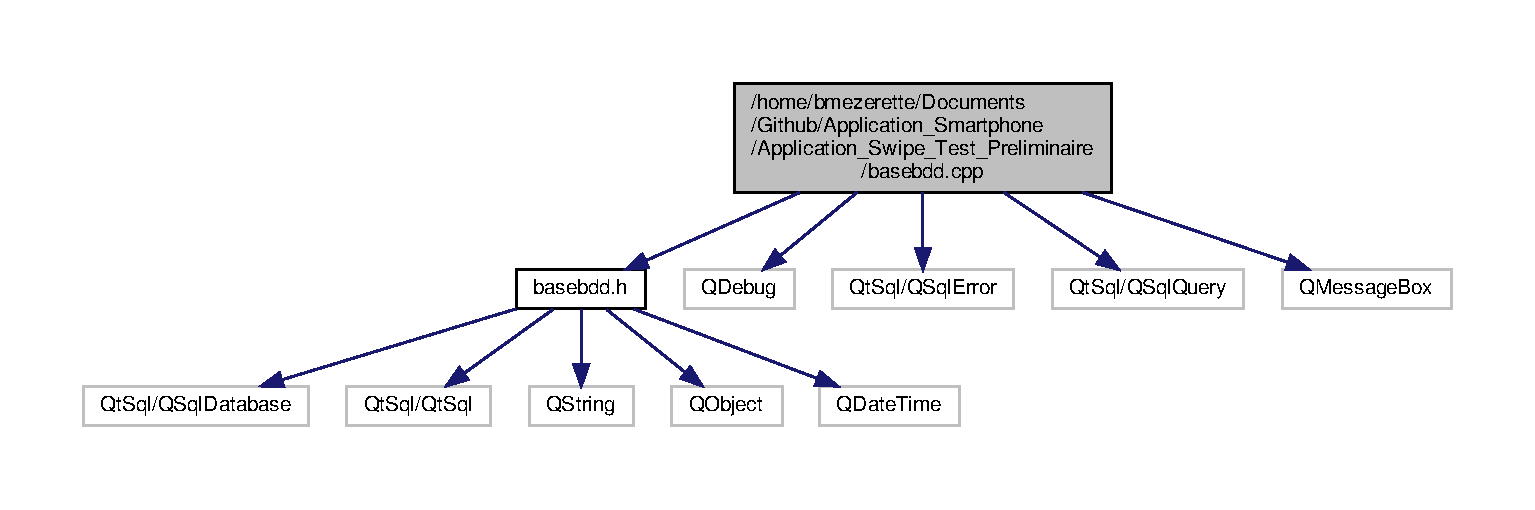
\includegraphics[width=350pt]{basebdd_8cpp__incl}
\end{center}
\end{figure}

\hypertarget{basebdd_8h}{}\section{Référence du fichier /home/bmezerette/\+Documents/\+Github/\+Application\+\_\+\+Smartphone/\+Application\+\_\+\+Swipe\+\_\+\+Test\+\_\+\+Preliminaire/basebdd.h}
\label{basebdd_8h}\index{/home/bmezerette/\+Documents/\+Github/\+Application\+\_\+\+Smartphone/\+Application\+\_\+\+Swipe\+\_\+\+Test\+\_\+\+Preliminaire/basebdd.\+h@{/home/bmezerette/\+Documents/\+Github/\+Application\+\_\+\+Smartphone/\+Application\+\_\+\+Swipe\+\_\+\+Test\+\_\+\+Preliminaire/basebdd.\+h}}
{\ttfamily \#include \char`\"{}Qt\+Sql/\+Q\+Sql\+Database\char`\"{}}\newline
{\ttfamily \#include $<$Qt\+Sql/\+Qt\+Sql$>$}\newline
{\ttfamily \#include $<$Q\+String$>$}\newline
{\ttfamily \#include $<$Q\+Object$>$}\newline
{\ttfamily \#include $<$Q\+Date\+Time$>$}\newline
Graphe des dépendances par inclusion de basebdd.\+h\+:
\nopagebreak
\begin{figure}[H]
\begin{center}
\leavevmode
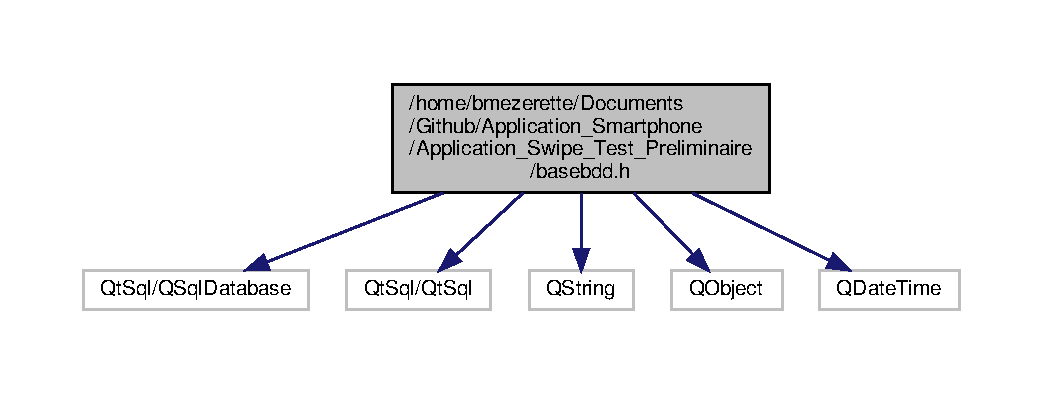
\includegraphics[width=350pt]{basebdd_8h__incl}
\end{center}
\end{figure}
Ce graphe montre quels fichiers incluent directement ou indirectement ce fichier \+:
\nopagebreak
\begin{figure}[H]
\begin{center}
\leavevmode
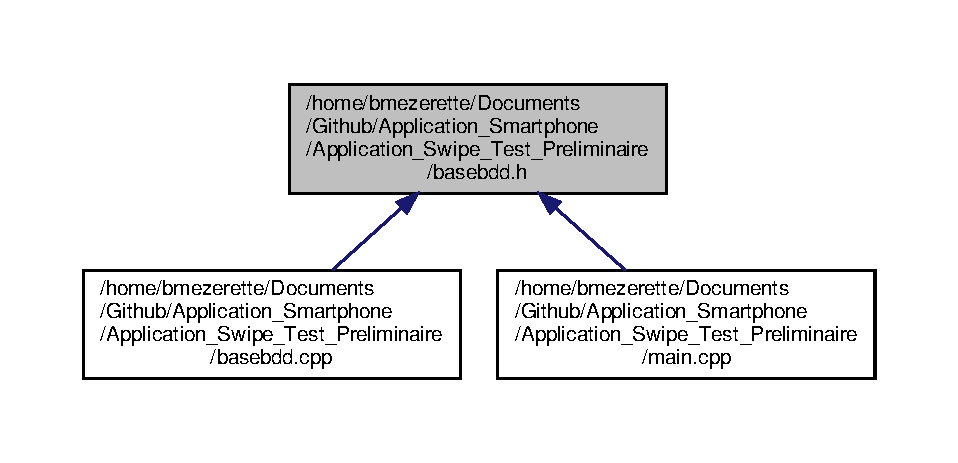
\includegraphics[width=350pt]{basebdd_8h__dep__incl}
\end{center}
\end{figure}
\subsection*{Classes}
\begin{DoxyCompactItemize}
\item 
class \hyperlink{class_base_b_d_d}{Base\+B\+DD}
\end{DoxyCompactItemize}

\hypertarget{main_8cpp}{}\section{Référence du fichier /home/bmezerette/\+Documents/\+Github/\+Application\+\_\+\+Smartphone/\+Application\+\_\+\+Swipe\+\_\+\+Test\+\_\+\+Preliminaire/main.cpp}
\label{main_8cpp}\index{/home/bmezerette/\+Documents/\+Github/\+Application\+\_\+\+Smartphone/\+Application\+\_\+\+Swipe\+\_\+\+Test\+\_\+\+Preliminaire/main.\+cpp@{/home/bmezerette/\+Documents/\+Github/\+Application\+\_\+\+Smartphone/\+Application\+\_\+\+Swipe\+\_\+\+Test\+\_\+\+Preliminaire/main.\+cpp}}
{\ttfamily \#include $<$Q\+Gui\+Application$>$}\newline
{\ttfamily \#include $<$Q\+Qml\+Application\+Engine$>$}\newline
{\ttfamily \#include $<$Qt\+Gui/\+Q\+Gui\+Application$>$}\newline
{\ttfamily \#include $<$Qt\+Qml/\+Q\+Qml\+Engine$>$}\newline
{\ttfamily \#include $<$Qt\+Quick/\+Q\+Quick\+View$>$}\newline
{\ttfamily \#include $<$Q\+Qml\+Context$>$}\newline
{\ttfamily \#include \char`\"{}basebdd.\+h\char`\"{}}\newline
Graphe des dépendances par inclusion de main.\+cpp\+:
\nopagebreak
\begin{figure}[H]
\begin{center}
\leavevmode
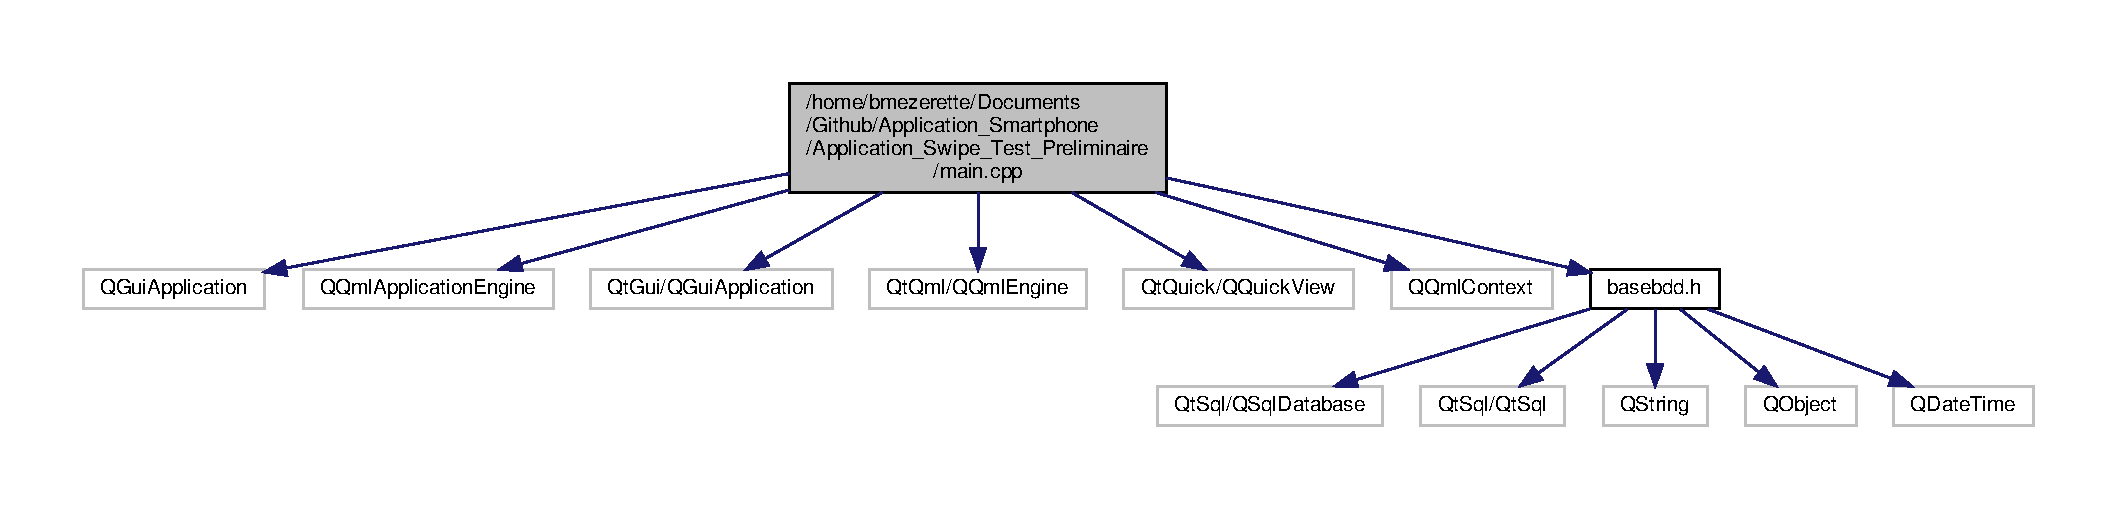
\includegraphics[width=350pt]{main_8cpp__incl}
\end{center}
\end{figure}
\subsection*{Fonctions}
\begin{DoxyCompactItemize}
\item 
int \hyperlink{main_8cpp_a0ddf1224851353fc92bfbff6f499fa97}{main} (int argc, char $\ast$argv\mbox{[}$\,$\mbox{]})
\end{DoxyCompactItemize}


\subsection{Documentation des fonctions}
\mbox{\Hypertarget{main_8cpp_a0ddf1224851353fc92bfbff6f499fa97}\label{main_8cpp_a0ddf1224851353fc92bfbff6f499fa97}} 
\index{main.\+cpp@{main.\+cpp}!main@{main}}
\index{main@{main}!main.\+cpp@{main.\+cpp}}
\subsubsection{\texorpdfstring{main()}{main()}}
{\footnotesize\ttfamily int main (\begin{DoxyParamCaption}\item[{int}]{argc,  }\item[{char $\ast$}]{argv\mbox{[}$\,$\mbox{]} }\end{DoxyParamCaption})}


%--- End generated contents ---

% Index
\backmatter
\newpage
\phantomsection
\clearemptydoublepage
\addcontentsline{toc}{chapter}{Index}
\printindex

\end{document}
